%%%  Ukázkový text a dokumentace stylu pro text závěrečné (bakalářské a
%%%  diplomové) práce na KI PřF UP v Olomouci
%%%  Copyright (C) 2012 Martin Rotter, <rotter.martinos@gmail.com>
%%%  Copyright (C) 2014 Jan Outrata, <jan.outrata@upol.cz>


%%  Pro získání PDF souboru dokumentu je třeba tento zdrojový text v
%%  LaTeXu přeložit (dvakrát) programem pdfLaTeX.

%%  V případě použití programu BibLaTeX pro tvorbu seznamu literatury
%%  je poté ještě třeba spustit program Biber s parametrem jméno
%%  souboru zdrojového textu bez přípony a následně opět (dvakrát)
%%  přeložit zdrojový text programem pdfLaTeX.

%%  Postup získání Postscriptového souboru je popsán v dokumentaci.


%%  Třída dokumentu implementující styl pro závěrečnou práci. Vybrané
%%  nepovinné parametry (ostatní v dokumentaci):

%%  'master' pro sazbu diplomové práce, jinak se sází bakalářská práce

%%  'field=kód' pro Váš studijní obor, kódy pro diplomovou práci 'uvt'
%%  pro Učitelství výpočetní techniky pro střední školy a 'binf' pro
%%  Bioinformatiku, jinak je výchozí Informatika, a pro bakalářskou
%%  práci 'ainfk' pro Aplikovanou informatiku v kombinované formě,
%%  'inf' pro Informatiku, 'infv' pro Informatiku pro vzdělávání a
%%  'binf' pro Bioinfomatiku, jinak je výchozí Aplikovaná informatika
%%  v prezenční formě

%%  'printversion' pro sazbu verze pro tisk (nebarevné logo a odkazy,
%%  odkazy s uvedením adresy za odkazem, ne odkazy do rejstříku),
%%  jinak verze pro prohlížeč

%%  'biblatex' pro zapnutí podpory pro sazbu bibliografie pomocí
%%  BibLaTeXu, jinak je výchozí sazba v prostředí thebibliography

%%  'language=jazyk' pro jazyk práce, jazyky english pro anglický,
%%  slovak pro slovenský, jinak je výchozí czech pro český

%%  'font=sans' pro bezpatkový font (Iwona Light), jinak výchozí
%%  patkový (Latin Modern)

\documentclass[
%  master,
  field=inf,
%  printversion,
  biblatex,
  language=english,
%  font=sans,
  glossaries,
  index
]{kidiplom}

%% Informace pro úvodní strany. V jazyku práce (pokud není v komentáři
%% uvedeno česky) a anglicky. Uveďte všechny, u kterých není v
%% komentáři uvedeno, že jsou volitelné. Při neuvedení se použijí
%% výchozí texty. Text pro jiný než nastavený jazyk práce (nepovinným
%% parametrem language makra \documentclass, výchozí český) se zadává
%% použitím makra s uvedením jazyka jako nepovinného parametru.

%% Název práce, česky a anglicky. Měl by se vysázet na jeden řádek.
\title[czech]{Vizualizace třídicích algoritmů}
\title[english]{Visualization of Sorting Algorithms}

%% Volitelný podnázev práce, česky a anglicky. Měl by se vysázet na
%% jeden řádek. Výchozí je prázdný.
%\subtitle{Ukázkový text a dokumentace stylu v \LaTeX{}u}
%\subtitle[english]{Sample text and documentation of the \LaTeX{} style}

%% Jméno autora práce. Makro nemá nepovinný parametr pro uvedení
%% jazyka.
\author{Mykhailo Klunko}

%% Jméno vedoucího práce (včetně titulů). Makro nemá nepovinný
%% parametr pro uvedení jazyka.
\supervisor{Mgr. Tomáš Kühr, Ph.D.}

%% Volitelný rok odevzdání práce. Výchozí je aktuální (kalendářní)
%% rok. Makro nemá nepovinný parametr pro uvedení jazyka.
%\yearofsubmit{\the\year}

%% Anotace práce, včetně anglické (obvykle překlad z jazyka
%% práce). Jeden odstavec!
\annotation[czech]{Cílem práce bylo vytvořit software pro podporu výuky třídících algoritmů pomocí vizualizace průběhu třídění nejznámějšími algoritmy a jejich variantami. Program byl vytvořen s podporou názorné vizualizaci vybraných algoritmů na zadaném či vygenerovaném vstupním poli a krokování průběhu výpočtu se souběžným zobrazením pseudokódu použitého algoritmu a aktuálních hodnot použitých proměnných.}

\annotation[english]{The main goal of the thesis was to create a learning support software with visualization of the most known sorting algorithms and their variations. The application has to support a graphic visualization of selected algorithms on randomly generated or manually created array, step-by-step execution possibility, pseudocode and current state of variables.}

%% Klíčová slova práce, včetně anglických. Oddělená (obvykle) středníkem.
\keywords[czech]{třídící algoritmus; třídění; vizualizace; program}
\keywords[english]{sorting algorithm; sorting; visualization; software}

%% Volitelná specifikace příloh textu práce, i anglicky. Výchozí je '1
%% CD/DVD'.
%\supplements{jedno kulaté placaté CD/DVD s malou kulatou dírou uprostřed}
%\supplements[english]{one round flat CD/DVD with a small round hole in the middle}

%% Volitelné poděkování. Stručné! Výchozí je prázdné. Makro nemá
%% nepovinný parametr pro uvedení jazyka.
\thanks{Děkuji, děkuji, děkuji.}

%% Cesta k souboru s bibliografií pro její sazbu pomocí BibLaTeXu
%% (zvolenou nepovinným parametrem biblatex makra
%% \documentclass). Použijte pouze při této sazbě, ne při (výchozí)
%% sazbě v prostředí thebibliography.
\bibliography{bibliografie.bib}
\addbibresource{bibliografie.bib}
%% Další dodatečné styly (balíky) potřebné pro sazbu vlastního textu
%% práce.
\usepackage{lipsum}
\usepackage{algorithm}
\usepackage{bm}

\begin{document}
%% Sazba úvodních stran -- titulní, s bibliografickými údaji, s
%% anotací a klíčovými slovy, s poděkováním a prohlášením, s obsahem a
%% se seznamy obrázků, tabulek, vět a zdrojových kódů (pokud jejich
%% sazba není vypnutá).
\maketitle

%% Vlastní text závěrečné práce. Pro povinné závěry, před přílohami,
%% použijte prostředí kiconclusions. Povinná je i příloha s obsahem
%% přiloženého CD/DVD.

%% -------------------------------------------------------------------

\newcommand{\BibLaTeX}{\textsc{Bib}\LaTeX}

%\noindent\textcolor{red}{\LARGE Upozornění: Následující text
%  dokumentace stylu, vyjma přílohy~\ref{sec:ObsahCD}, je rozpracovaná
%  a (značně) neúplná verze!!!}

\section{Introduction}

Nowadays sorting algorithms are widely used in software. For example if you open file explorer on your PC, you may see files sorted in different ways. Students of computer science start learning different algorithms in the first year of studies and sorting algorithms are among them.

The main goal of the thesis was to create a program which would serve as a tool for understanding how most known sorting algorithms work. Since I faced the problems of sorting during the course of algorithm design, now there is understanding that the visual representation is a vital part of studying process.

Text of the thesis describes principles of some basic sorting algorithms.  



\subsection{Usage of sorting algorithms?}

\subsection{Visual solution}

\subsection{Přepínače}
Styl kidiplom je z hlediska uživatele zastoupen ekvivalentně nazvanou třídou, kterou je třeba volat na záčátku dokumentu:


Následuje přehled přepínačů, je vždy uvedeno jméno přepínač, včetně výchozí hodnoty. Přepínače uvádí tabulka \ref{tab:prepinace}.

\subsection{Geometrie stránky}
Tento styl používá list velikosti $A4$. Pro sazbu prací je třeba použít jednostrannou sazbu. Levý okraj je rozšířen s ohledem na vazbu výsledné knižní podoby práce.

\section{Algorithms}

This section describes algorithms represented in the program.

\subsection{Insertion Sort}

Insertion sorting algorithm has a simple idea. Assume the items to be sorted. We divide the items into two parts: sorted one and unsorted one. Usually at the beginning sorted part consists of the first element. Then for the each next step we take one item from the unsorted part and insert it into the right place among the sorted items.
\begin{figure}[H]
\begin{center}
	
	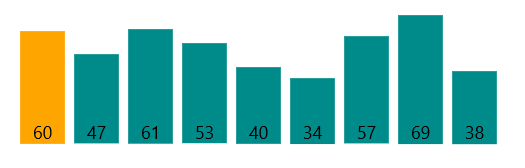
\includegraphics[scale=0.7]{img/Insertion.png}
	\caption{Insertion Sort at start}\label{fig:insert}
\end{center}
\end{figure}


\subsection{Selection Sort}
\label{sec:selection}

Selection Sort is based on the repeated selection. As well as in the Insertion Sort, here we have sorted part and unsorted part.

Assume an array of items. At the beginning of sorting process unsorted part is represented by the whole array. Then the first item of the unsorted part is set as the smallest key and is compared with the follow-up elements. When smaller item is found, it is set as a new smallest key. After the end of the array is reached the smallest item is swapped with the first unsorted  element and it becomes the sorted part of the array. This step is repeated till the array is sorted.

\subsection{Bubble Sort}

At the base of the Bubble Sort lies the idea of exchanging two adjacent elements if they are in wrong order. Algorithm works stepping through the all elements so the largest element tends to move to the right.

Now we are going to the details. Let us have an array to sort. Algorithm does $n$ iterations where $n$ is equal to the size of array. And at the end of each iteration through the array the range of inspected items gets smaller till it becomes zero.

It happens because during each iteration as it was already mentioned for ascending order the largest element of current range "bubbles" to the end.

Repeating such iterations we receive each element into its right position.

%add pic of bubblesort in action
\subsection{Cocktail Sort}

Cocktail Sort or also known as Bidirectional Sort. This algorithm similarly to the Bubble Sort uses the idea of exchanging unordered adjacent items of array. 

Assume array that needs to be sorted in ascending order. Above we described Bubble Sort and this algorithm has a significant problem. It iterates through array only in one direction. This way, smaller items which are closer to the end of array reach its right positions slowly.

Solution is to make Bubble Sort iterate left-to-right and right-to-left. Cocktail Sort uses two cycles inside a big one:

\begin{enumerate}
 \item Iterate from $a$ to $b$, compare adjacent elements and swap if they are not ordered.
 \item Iterate from $b$ to $a + 1$ same way as in the step $1$
 \item Repeat steps 1. and 2. but with a bit different range from $a = a + 1$ to $b = b - 1$
\end{enumerate}

\subsection{Quick Sort}

Quick Sort works on the principle "divide and conquer". It recursively applies itself on smaller parts of array until it is not sorted.

Algorithm takes one item at unsorted array or its part, usually it is the leftmost or the rightmost element of array. Then this item also known as pivot is moved to its final position in the array that is should occupy. While determining pivot's position, other elements of array are rearranged the way that no bigger elements on the right and no smaller elements are on the left.

This way, it is enough to apply Quick Sort on each part of array not including pivot until array is not sorted.

\begin{figure}[H]
\begin{center}
	
	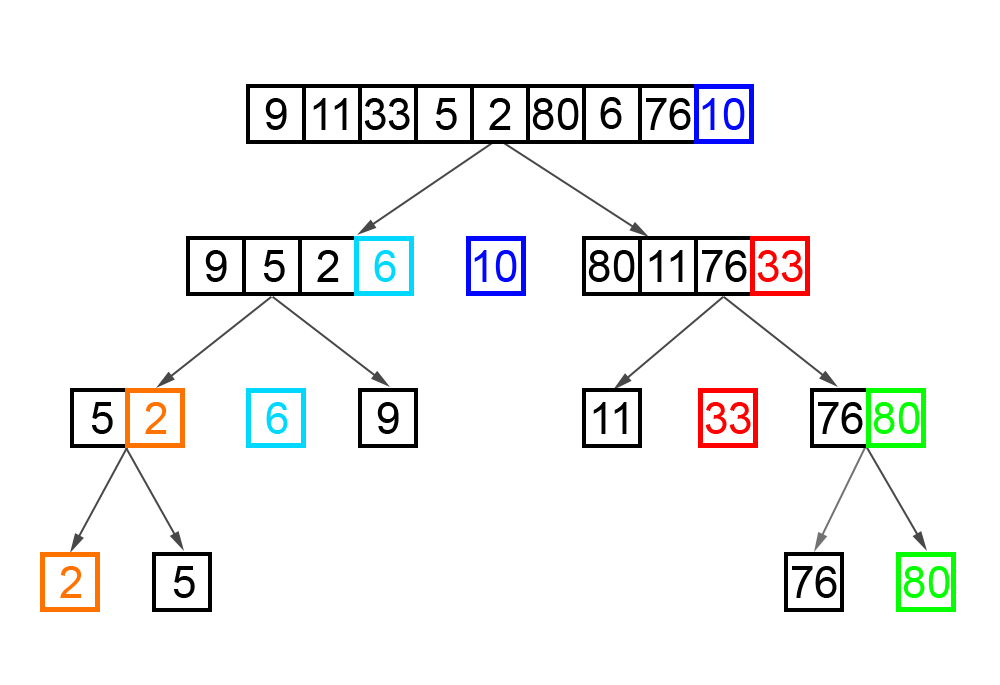
\includegraphics[scale=0.7]{img/Quicksort.png}
	\caption{Quick Sort principle}\label{fig:insert}
\end{center}
\end{figure}

There are several methods of partitioning of array into two parts, here I want to describe one that is demonstrated in the software part of this work.

Firstly, a pivot and index item are selected on the unsorted array or its part. Assume pivot is the last item and index is the first. Next each item of array except pivot is compared with the pivot. If current item is lesser or equal to pivot, it is swapped with the index item, next in order item becomes index. Finally, index and pivot are swapped and this way pivot is on its final position.

\subsection{Merge Sort}

Merge Sort as well as Quick Sort is an algorithm of type "divide and conquer". The logic of it is simple: recursively divide data into two parts till it becomes indivisible then merge parts back.

Merge procedure itself takes items from each previously divided part one by one, compares them and moves the smallest to the output, repeats previous step.

\begin{figure}[H]
\begin{center}
	
	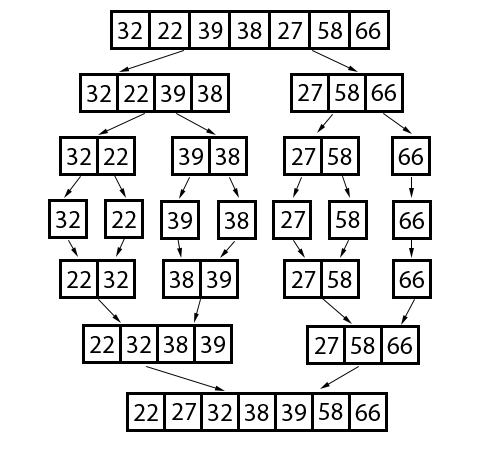
\includegraphics[scale=2.5]{img/Mergesort.png}
	\caption{Merge Sort principle}\label{fig:insert}
\end{center}
\end{figure}

\subsection{Heap Sort}

Heap Sort is a selection based algorithm and it offers another interesting approach to sorting. In comparison with the \hyperref[sec:selection]{Selection Sort} it has optimized selection by using binary heap data structure. 

Binary heap is a complete binary tree; it means that all levels of tree, except the last one, must be completely filled with nodes. Also, this data structure satisfies the \textit{heap condition}: each node key is greater than or equal to its child keys (this heap type is called \textit{max-heap}).

\begin{figure}[H]
\begin{center}
	
	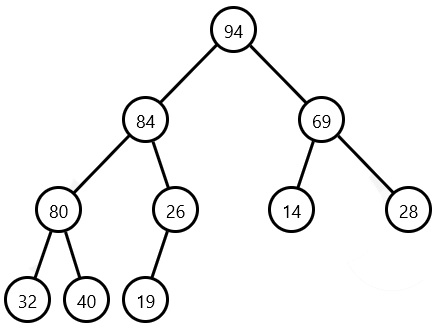
\includegraphics[scale=0.7]{img/Maxheap.png}
	\caption{Max-Heap}\label{fig:maxheap}
\end{center}
\end{figure}

Binary heap may be implemented by simple array. Item at position zero is a root node, items at position one and two are respectively left and right children of the root. From that representation it is easy to find children of each node (if they exist). Assume a node at position $k$ then its left child is at $2k + 1$ and its right child is at $2k + 2$.

\begin{figure}[H]
\begin{center}
	
	
\includegraphics[scale=3]{img/Heapsort.png}
	\caption{Children positions in heap}\label{fig:heapsort}
\end{center}
\end{figure}

\textbf{Heap Sort itself works as follows:}
\begin{enumerate}
 \item \label{itm:step1} Build max-heap
 \item \label{itm:step2} Swap root and the last node, reduce size of heap by one
 \item \label{itm:step3} Build max-heap without the node on a reduced position
 \item Repeat steps \ref{itm:step2} and \ref{itm:step3} until the range of array is one
\end{enumerate}

To build \textit{max-heap} from current node we need to assure that right and left child comprise max-heaps. This way, in the first step procedure for building max-heap is recursively applied for each node that has at least one child from bottom to top.

After each swap of the root node and the node at last considered position last node takes its final place. This way it joins the sorted part of array.

Worst and average case complexity of Heap Sort are both $\bm{\Theta(n \log(n))}$.

\subsection{Counting Sort}

Counting Sort is usually used for sorting keys in some range. Algorithm is based on counting keys of distinct values. Final positions of keys are calculated from the previous computations.

Assume we have integers in range from $0$ to $k$.

\subsection{Radix Sort}

\subsection{Bucket Sort}

\section{Documentation}

\section{User Guide}

%% Závěry práce. V jazyce práce a anglicky. Text pro jiný než
%% nastavený jazyk práce (nepovinným parametrem language makra
%% \documentclass, výchozí český) se zadává použitím makra s uvedením
%% jazyka jako nepovinného parametru.
\begin{kiconclusions}
Závěr práce v \uv{českém} jazyce.
\end{kiconclusions}

\begin{kiconclusions}[english]
Thesis conclusions in \uv{English}.
\end{kiconclusions}

%% Přílohy obsahu textu práce, za makrem \appendix.
\appendix

\section{První příloha}
Text první přílohy

\section{Druhá příloha}
Text druhé přílohy

%% Obsah přiloženého CD/DVD. Poslední příloha. Upravte podle vlastní
%% práce!
\section{Obsah přiloženého CD/DVD} \label{sec:ObsahCD}

Na samotném konci textu práce je uveden stručný popis obsahu
přiloženého CD/DVD, tj.~jeho závazné adresářové struktury, důležitých
souborů apod.

\begin{description}

\item[\texttt{bin/}] \hfill \\
  Instalátor \textsc{Instalator} programu, popř.~program
  \textsc{Program}, spustitelné přímo z~CD/DVD. / Kompletní adresářová
  struktura webové aplikace \textsc{Webovka} (v~ZIP archivu) pro
  zkopírování na webový server. Adresář obsahuje i~všechny runtime
  knihovny a~další soubory potřebné pro bezproblémový běh instalátoru
  a~programu z~CD/DVD / pro bezproblémový provoz webové aplikace na
  webovém serveru.

\item[\texttt{doc/}] \hfill \\
  Text práce ve formátu PDF, vytvořený s~použitím závazného stylu KI
  PřF UP v~Olomouci pro závěrečné práce, včetně všech příloh,
  a~všechny soubory potřebné pro bezproblémové vygenerování PDF
  dokumentu textu (v~ZIP archivu), tj.~zdrojový text textu, vložené
  obrázky, apod.

\item[\texttt{src/}] \hfill \\
  Kompletní zdrojové texty programu \textsc{Program} / webové aplikace
  \textsc{Webovka} se všemi potřebnými (příp.~převzatými) zdrojovými
  texty, knihovnami a~dalšími soubory potřebnými pro bezproblémové
  vytvoření spustitelných verzí programu / adresářové struktury pro
  zkopírování na webový server.

\item[\texttt{readme.txt}] \hfill \\
  Instrukce pro instalaci a~spuštění programu \textsc{Program}, včetně
  všech požadavků pro jeho bezproblémový provoz. / Instrukce pro
  nasazení webové aplikace \textsc{Webovka} na webový server, včetně
  všech požadavků pro její bezproblémový provoz, a~webová adresa, na
  které je aplikace nasazena pro účel testování při tvorbě posudků
  práce a~pro účel obhajoby práce.

\end{description}

Navíc CD/DVD obsahuje:

\begin{description}

\item[\texttt{data/}] \hfill \\
  Ukázková a~testovací data použitá v~práci a~pro potřeby testování
  práce při tvorbě posudků a~obhajoby práce.

\item[\texttt{install/}] \hfill \\
  Instalátory aplikací, runtime knihoven a~jiných souborů potřebných
  pro provoz programu \textsc{Program} / webové aplikace
  \textsc{Webovka}, které nejsou standardní součástí operačního
  systému určeného pro běh programu / provoz webové aplikace.

\item[\texttt{literature/}] \hfill \\
  Vybrané položky bibliografie, příp.~jiná užitečná literatura
  vztahující se k~práci.

\end{description}

U~veškerých cizích převzatých materiálů obsažených na CD/DVD jejich
zahrnutí dovolují podmínky pro jejich šíření nebo přiložený souhlas
držitele copyrightu. Pro všechny použité (a~citované) materiály,
u~kterých toto není splněno a~nejsou tak obsaženy na CD/DVD, je uveden
jejich zdroj (např.~webová adresa) v~bibliografii nebo textu práce
nebo v souboru \texttt{readme.txt}.

%% -------------------------------------------------------------------

%% Sazba volitelného seznamu zkratek, za přílohami.
\printglossary

%% Sazba povinné bibliografie, za přílohami (případně i za seznamem
%% zkratek). Při použití BibLaTeXu použijte makro
%% \printbibliography. jinak prostředí thebibliography. Ne obojí!

%% Sazba i v textu necitovaných zdrojů, při použití
%% BibLaTeXu. Volitelné.
\nocite{*}
%% Vlastní sazba bibliografie při použití BibLaTeXu.
\printbibliography

%% Bibliografie, včetně sazby, při nepoužití BibLaTeXu.
% \begin{thebibliography}{9}
%\bibitem{kniha2} \uppercase{Hawke}, Paul. NanoHttpd: Light-weight HTTP server designed for embedding in other applications. GitHub [online]. 2014-05-12. [cit. 2014-12-06]. Dostupné z: \url{https://github.com/NanoHttpd/nanohttpd}
%
%\bibitem{jeske13} \uppercase{Jeske}, David; \uppercase{Novák}, Josef. Simple HTTP Server in \csharp: Threaded synchronous HTTP Server abstract class, to respond to HTTP requests. CodeProject: For those who code [online]. 2014-05-24. [cit. 2014-12-06]. Dostupné z: \url{http://www.codeproject.com/Articles/137979/Simple-HTTP-Server-in-C}
%
%\bibitem{uzis2012} \uppercase{ÚSTAV ZDRAVOTNICKÝCH INFORMACÍ A STATISTIKY ČR}. Lékaři, zubní lékaři a farmaceuti 2012 [online]. Praha 2, Palackého náměstí 4: Ústav zdravotnických informací a statistiky ČR, 2012 [cit. 2014-12-06]. ISBN 978-80-7472-089-5. Dostupné z: \url{http://www.uzis.cz/publikace/lekari-zubni-lekari-farmaceuti-2012}
% \end{thebibliography}

%% Sazba volitelného rejstříku, za bibliografií.
\printindex

\end{document}
